\chapter{Controlador de corriente} \chapterlabel{Informe/4-ControladorCorriente} \label{cap:ControladorCorriente}
\section{Diseño y modelado}

\noindent Para regular la fuerza ejercida por el electroimán es necesario controlar la corriente que circula por él. Para ello, se modela a la planta como la impedancia de un inductor con una resistencia serie, cuya inductancia varía con el gap de aire:

\begin{equation} \label{eq_admitancia}
\frac{1}{sL(y)\ +\ R_L}
\end{equation}

\noindent Para realizar este control se utiliza un sistema realimentado, como el que se muestra en la figura \ref{fig:img_diag-en-bloques}. Se puede ver que se ingresa con una tensión de referencia ($V_{in}$) proporcional a la corriente de salida deseada, que luego se multiplica por la ganancia de entrada ($K_{in}$). La corriente del electroimán se realimenta en forma de una tensión proporcional a ella ($V_{iF}$). Ambas tensiones son restadas y el resultado (e) ingresa al bloque de comparador con histéresis, que actúa en conmutación, por lo que su salida tiene dos estados posibles: $\pm$$V_L$.

\noindent Al ser aplicadas al inductor se producirá una rampa de corriente: si la tensión es positiva, la rampa crece, y si es negativa decrece. De esta forma, debido a la conmutación del comparador se obtiene, a la salida, una forma de onda triangular $I_L$, cuyo valor medio es la corriente deseada y se corresponde a la tensión de referencia.

\begin{figure}[H]
	\centering
	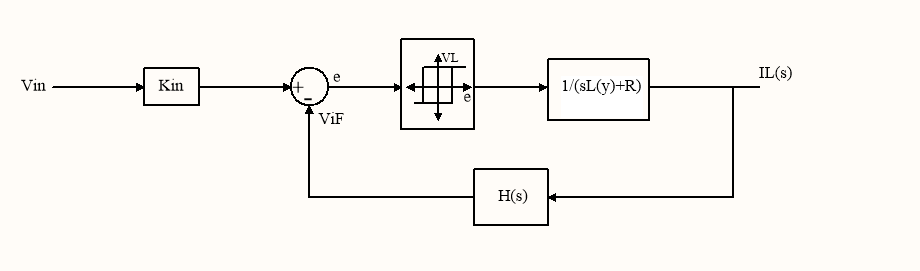
\includegraphics[width=\textwidth]{Diagrama-en-bloques.png}
	\caption{Diagrama en bloques simplificado del controlador de corriente.}
	\label{fig:img_diag-en-bloques}
\end{figure}

\subsection{Características del sistema}

\begin{itemize}
    \item Para sensar la corriente se utiliza un sensor de efecto Hall HO 15-NP, con una transconductancia de H(s) = 53.3 mV/A.
    \item Para la ganancia de entrada $K_{in}$ se utiliza un valor de 0.32 puesto que $V_{in}$ varía entre 0 V y 5 V y debe mapearse con una corriente variable entre 0 A y 30 A.
    \item Se adopta una variación de la corriente en torno a su valor medio (ripple) de 500 mA, por lo que resulta en un ancho de histéresis de 26.665 mV.
    \item Según mediciones realizadas sobre el electroimán, la inductancia en el punto de equilibrio $Y_0=\:4mm$ es de 16.44 mHy (considerando la inductancia de dispersión de 8.89 mHy) y la resistencia serie es de 0.2 $\Omega$.
    \item La tensión aplicada sobre el electroimán es +24 V para el estado ON y -24 V para el estado OFF.
    \item Se utiliza un driver de corriente que trabaja en conmutación mediante un puente H con 4 N-MOS. 
\end{itemize}

\subsection{Circuito del controlador de corriente}

\noindent Se plantea la etapa de entrada que consiste en la ganancia $K_{in}$ y el restador con la realimentación. El objetivo es imponer una ganancia de entrada de 0.32, y que la salida de esta etapa tenga un punto de operación de $2.5\:V$ para poder utilizar una fuente de alimentación entre $0\:V$ y $5\:V$ para los operacionales. Para lograr esto se utiliza un circuito como el que se muestra en la figura \ref{fig:img_etapa-de-entrada}.

\begin{figure}[H]
	\centering
	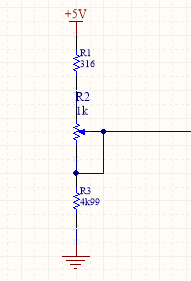
\includegraphics[scale=1]{Etapa-de-entrada.png}
	\caption{Etapa de entrada.}
	\label{fig:img_etapa-de-entrada}
\end{figure}

\noindent Para la implementación del comparador con histéresis se utiliza un amplificador operacional realimentado positivamente. Se implementa un ancho de histéresis de 26.665 mV,  alrededor de un punto de operación de 2.5 V, como se muestra en la figura \ref{fig:img_comp-con-hist}.

\begin{figure}[H]
	\centering
	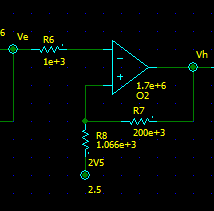
\includegraphics[scale=1]{Comparador-con-histeresis.png}
	\caption{Comparador con histéresis.}
	\label{fig:img_comp-con-hist}
\end{figure}

\noindent Para controlar la corriente en el electroimán se utiliza una topología en puente H, que permite conmutar la polaridad de la tensión aplicada a la bobina. Para medir la corriente se utiliza un sensor de efecto Hall, que es modelado en la simulación como  una fuente de tensión controlada por corriente, con una ganancia de 53.3 mV/A correspondiente a su transconductancia. Esta implementación puede observarse en la figura \ref{fig:img_puenteH}. A continuación, su salida es realimentada a la etapa de entrada luego de restarle la tensión de referencia  $V_{bias}$ de 2.5V, como se muestra en la figura \ref{fig:img_resta-Vbias}. 

\begin{figure}[H]
	\centering
	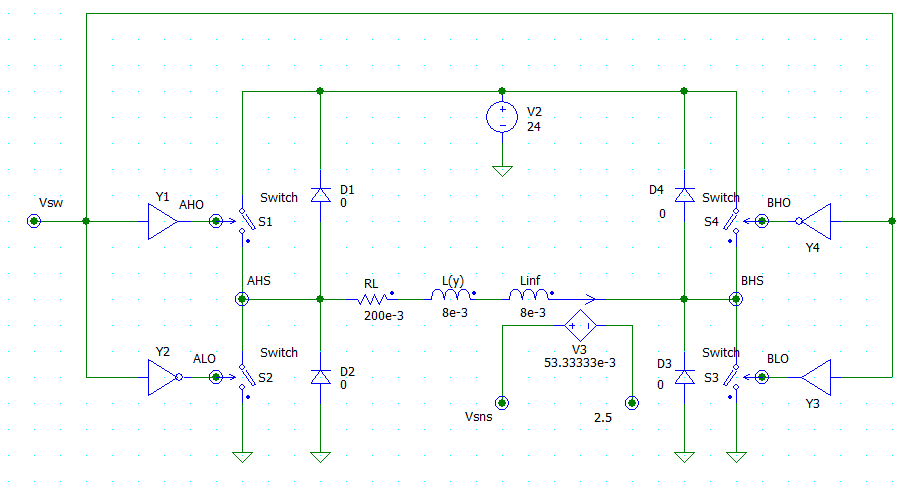
\includegraphics[scale=0.5]{PuenteH.png}
	\caption{Puente H y sensor de efecto Hall.}
	\label{fig:img_puenteH}
\end{figure}

\begin{figure}[H]
	\centering
	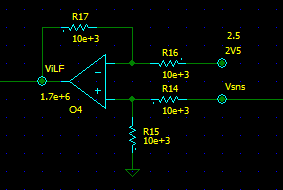
\includegraphics[scale=1]{Resta-Vbias.png}
	\caption{Resta del $V_{bias}$ al sensor de efecto Hall.}
	\label{fig:img_resta-Vbias}
\end{figure}

\subsubsection{Simulaciones de formas de onda}

\noindent En la figura \ref{fig:img_formas-de-onda-corriente} se pueden observar dos formas de onda. La inferior  corresponde a la tensión de salida del comparador con histéresis y la superior a la corriente que circula por el electroimán. Para la simulación se utilizó una tensión de referencia de entrada de 1 V, por lo que el valor medio de la corriente en la salida es 6 A con un ripple de 500 mA.

\begin{figure}[H]
	\centering
	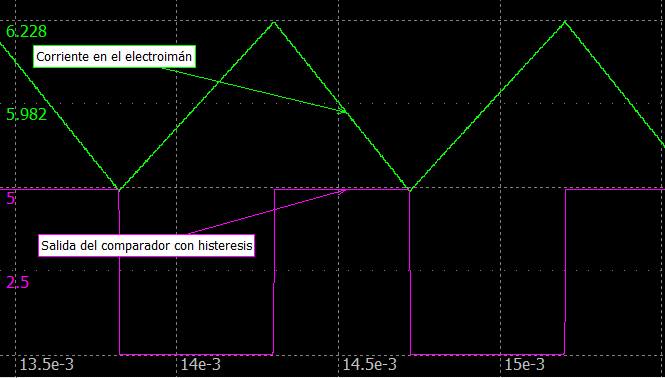
\includegraphics[scale=0.5]{Formas-de-onda-corriente.png}
	\caption{Formas de onda de corriente en el electroimán y tensión de salida del comparador.}
	\label{fig:img_formas-de-onda-corriente}
\end{figure}



\subsubsection{Simulación de un escalón en la referencia de corriente}

\noindent En la figura \ref{fig:img_respuesta-al-escalon} se muestra cómo cambia la corriente en el electroimán al aplicarle a la entrada del controlador un escalón de tensión entre 1 V y 3 V. Se puede observar cómo la conmutación del comparador se detiene para ajustar la corriente con la referencia.

\begin{figure}[H]
	\centering
	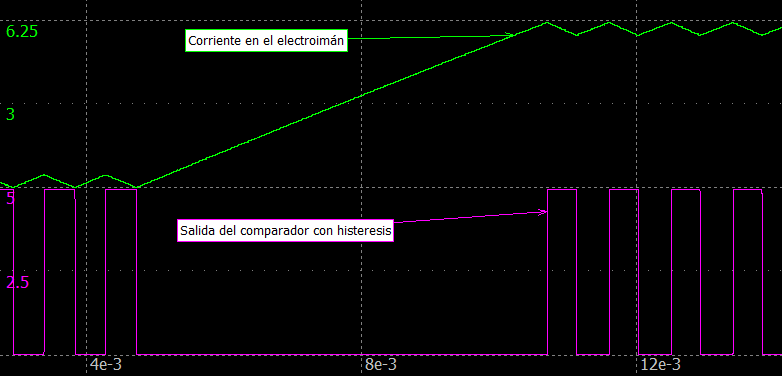
\includegraphics[scale=0.5]{Respuesta-al-escalon.png}
	\caption{Respuesta al escalón del circuito.}
	\label{fig:img_respuesta-al-escalon}
\end{figure}


\subsubsection{Descripción general de la topología}

\noindent Se desea controlar la corriente que circula por el electroimán y, debido a que el sistema va a trabajar con corrientes elevadas, es importante que la implementación del controlador de corriente sea eficiente. Por lo tanto, para disminuir la disipación de potencia del circuito se utiliza un controlador que funciona en conmutación. 

\noindent Para lograr una corriente contínua en el electroimán mediante una fuente conmutada se debe alternar la polaridad de la tensión aplicada en los bornes del inductor. De esta forma, la corriente crece y decrece (según la polaridad) con forma exponencial debido a la resistencia interna del electroimán. Sin embargo, como el intervalo de tiempo de esta conmutación es pequeño comparado con la constante de tiempo de la planta, el incremento de corriente será pequeño y puede ser aproximado a una recta. Por lo tanto se obtiene una corriente contínua con un ripple superpuesto de forma triangular. 

\noindent Para lograr alternar la polaridad de la fuente sobre el inductor se utiliza una topología en puente H con 4 MOSFET que funcionan con un ciclo de trabajo determinado (manejado por el controlador por histéresis) como se observa en la figura \ref{fig:img_topologia-puenteH}. Pueden diferenciarse dos semiciclos de trabajo: uno de estado ON y otro de estado OFF. El primero se define como el semiciclo durante el cual la corriente en el inductor crece (pendiente positiva), mientras que el segundo se da cuando la corriente decrece.

\begin{figure}[H]
	\centering
	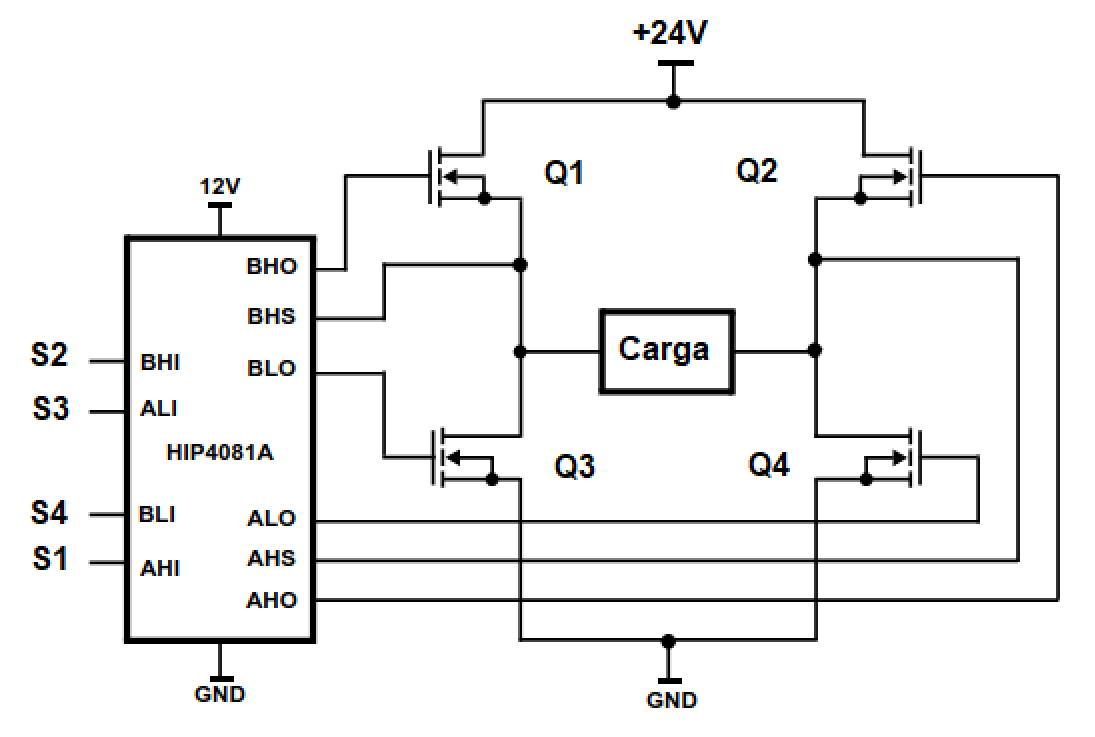
\includegraphics[scale=0.7]{Topologia-puenteH.png}
	\caption{Topología elemental del puente H.}
	\label{fig:img_topologia-puenteH}
\end{figure}

\noindent El electroimán se conecta entre los puntos medios de cada par de transistores. De esta manera se puede conmutar la polaridad de la tensión que se le aplica. Sólo se permite que dos transistores se enciendan a la vez, y esto se realiza de manera diagonal. Es decir, en la figura \ref{fig:img_topologia-puenteH}, Q1 y Q4 pueden estar encendidos, mientras que Q3 y Q2 están apagados, y viceversa. De otra forma, se podría generar un cortocircuito entre la fuente de alimentación y GND, que produciría una circulación de corriente denominada shoot-through. 


\noindent Los cuatro MOSFET utilizados para el puente H son de tipo N. Para que estos puedan funcionar correctamente en conmutación es necesario que en el estado ON, la diferencia de tensión entre gate y source sea mayor o igual a 7 V. Esto no es un problema para los dos MOS inferiores del puente H (Q2 y Q4), ya que la tensión en source está fijada en GND y el driver puede aplicar 12 V al gate (superando los 7 V entre gate y source). El problema radica en los transistores superiores del puente H, ya que la tensión en source varía entre 0 V y 24 V, por lo que en el gate debería haber, por lo menos, 31 V con respecto a GND. Sin embargo, la tensión máxima disponible entregada por la fuente es de 24 V. Para resolver este problema se utiliza un driver flotante con bootstrap.

\noindent Para controlar la conmutación se utiliza un mosfet driver HIP4081A \colorbox{yellow}{datasheet o algo?} que se encarga de encender y apagar los transistores según las entradas de control. Además permite la configuración de un tiempo muerto para evitar que se enciendan dos transistores de un lado a la vez. También provee la circuitería necesaria para implementar la fuente flotante que enciende los mosfet del lado superior para lo cual solo se debe agregar un diodo y un capacitor de manera externa. Para la implementación circuital se van a utilizar los MOSFET IPB160N04.\colorbox{yellow}{datasheet o algo?}

\noindent En la figura \ref{fig:img_bootstrap} se observa solo una de las mitades del puente H (lado A)  junto con las señales de control provistas por el driver HIP4081A\colorbox{yellow}{aclaramos tomadas del datasheet?}. El análisis para la otra mitad es análogo, por lo que se evita por simplicidad. La implementación del driver bootstrap permite obtener en el gate del MOS superior, una tensión de 36 V respecto a GND, logrando así una diferencia de tensión mayor a 7 V entre gate y source. 

\begin{figure}[H]
	\centering
	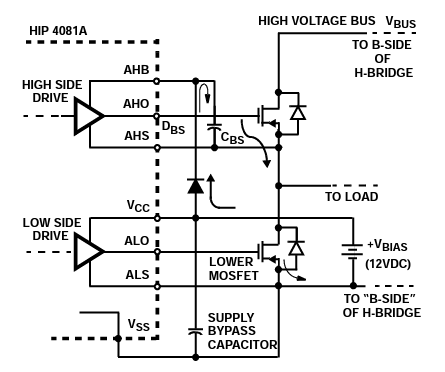
\includegraphics[scale=0.7]{Bootstrap.png}
	\caption{Configuración Bootstrap simplificada.}
	\label{fig:img_bootstrap}
\end{figure}

\noindent El driver bootstrap consiste en un capacitor ($C_{BS}$), un diodo, y la circuitería interna del HIP4081A. Para garantizar el correcto funcionamiento del bootstrap, al encender el sistema, la secuencia de inicio del HIP4081A enciende las dos salidas de la parte inferior del puente H: ALO y BLO con el fin de encender Q2 y Q4 durante un tiempo que se conoce como periodo de refresco de bootstrap. De esta forma, los capacitores de bootstrap de ambos lados quedan conectados entre $12 \:V$ y GND y se pueden cargar completamente. Durante este tiempo, las salidas a los gates AHO y BHO se mantienen en bajo continuamente lo que asegura que no se produzca corriente de shoot-through durante el período nominal de refresco del bootstrap. Una vez finalizado, las salidas responden normalmente al estado de las señales de entrada de control.

\noindent Para comprender su funcionamiento se hará un breve análisis del sistema. Para ello, se parte suponiendo que el sistema se encuentra funcionando: con el transistor Q2 encendido (ALO = $V_{CC}$), Q1 apagado (AHO = AHS = 0 V) y la corriente circulando de izquierda a derecha como lo indica la figura \ref{fig:img_bootstrap}. En ese caso, el capacitor $C_{BS}$ se carga a 12 V, ya que en un terminal tiene la fuente de 12 V (a través del diodo $D_{BS}$) y el otro está conectado a GND por medio de Q2.

\noindent Una vez que se apaga el transistor inferior, empieza a transcurrir el tiempo muerto. Teniendo en cuenta que la carga es inductiva, el valor medio de la corriente mantiene su sentido circulando por los diodos antiparalelos del MOS inferior del lado A y el superior del lado B. Esto provoca que el source del MOS superior del lado A tenga una tensión negativa igual a la caída de tensión en directa del diodo antiparalelo de Q2. 

\noindent Una vez finalizado el tiempo muerto, se enciende el MOS Q1. Para encenderlo, la señal AHO se pone en nivel alto. Durante el tiempo que Q1 pasa de estar apagado a encendido, la tensión en el source cambia de $-V_d$ a $V_{bus}$ de manera gradual mientras se carga el gate, y AHO pasa a ser igual a AHB, que es igual a la tensión entregada por el capacitor de bootstrap sumada a la tensión en el source de Q1. De esta manera se logra una tensión de 36 V con respecto a GND en el gate y genera una diferencia entre gate y source de 12 V.

\noindent Para lograr un funcionamiento adecuado del Boostrap es necesario dimensionar correctamente al capacitor $C_{BS}$ con el fin de que pueda proveer la carga suficiente durante el tiempo en el que el MOS esté encendido.


\subsubsection{Dimensionamiento de capacitor de bootstrap}

\noindent Para el dimensionamiento de los capacitores de bootstrap se tuvieron en cuenta sugerencias y procedimientos descriptos en \cite{HIP4081A_AN9405} y \cite{HIP4081A_FN3659}.
\colorbox{yellow}{Chequear si esto es cierto}	

\noindent Para encender un NMOS es necesario proveer corriente a su gate hasta cargar las capacidades parásitas entre gate-source y gate-drain. Una vez cargadas, el MOS queda en estado encendido y no consume más corriente en el gate. En el caso de los MOS del lado superior, esta corriente proviene del capacitor de bootstrap. 

\noindent En la implementación del puente H se decidió colocar resistencias entre gate y source, que aparecen como R1, R2, R3 y R4 en la figura \ref{fig:img_capacitores-puenteH}, \colorbox{yellow}{cuyo propósito se explica en la sección [3.1.2.4.1]}. Debido a la diferencia de tensión entre gate-source, se genera una corriente constante en estas resistencias durante el tiempo que el MOS esté encendido, que también debe ser provista por el  bootstrap.

\begin{figure}[H]
	\centering
	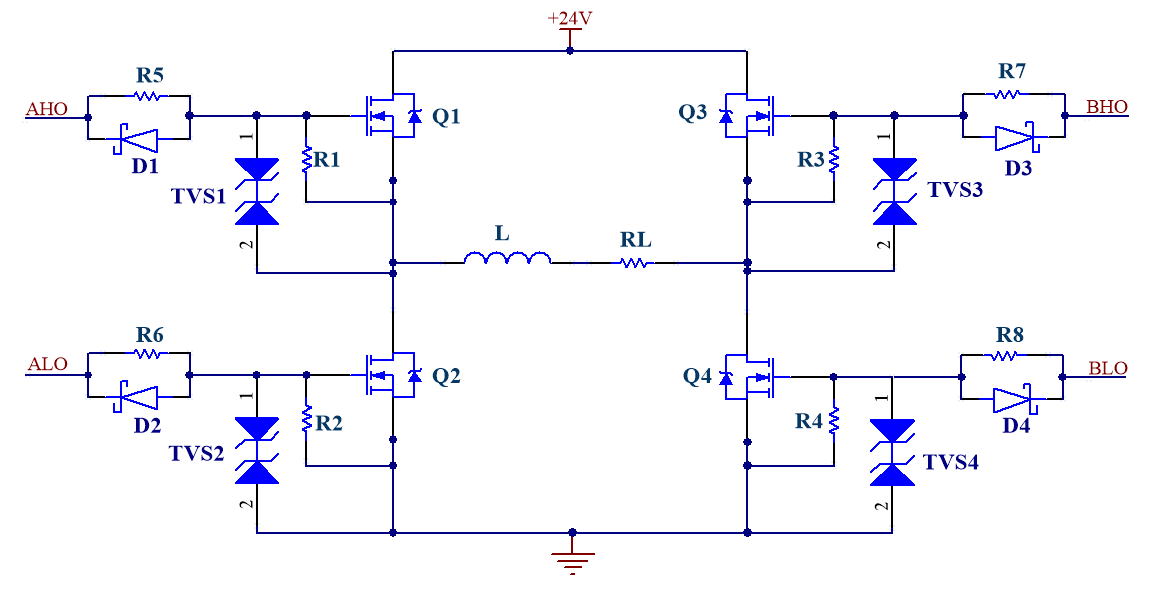
\includegraphics[scale=0.5]{Capacitores-puenteH.png}
	\caption{Puente H.}
	\label{fig:img_capacitores-puenteH}
\end{figure}

\noindent Por otro lado, el capacitor debe entregar corriente al diodo de bootstrap cuando este queda en inversa ($I_{DR}$ ), y también entregar una corriente de fuga al circuito integrado HIP ($I_{QBS}$ ). Esta última se desprecia ya que es compensada internamente por la bomba de carga del HIP.

\noindent Por lo tanto, para poder dimensionar correctamente el capacitor de bootstrap es necesario tener en cuenta todos los efectos mencionados anteriormente. Para ello se parte planteando la carga que almacena el capacitor bootstrap:

\begin{equation} \label{eq_carga-cap-bootstrap}
Q_{BS}=C_{BS}*\Delta V_{BS}
\end{equation}

\noindent En la ecuación \ref{eq_carga-cap-bootstrap}, $Q_{BS}$ es la carga total del capacitor de bootstrap, $C_{BS}$ su capacidad, y $\Delta V_{BS}$ es la diferencia de  tensión entre sus terminales. 

\noindent Para evitar sufrir una caída de tensión tal que afecte el encendido de los MOS, es necesario que $Q_{BS}$ pueda abastecer también al gate, al diodo en inversa y a la resistencia entre gate-source. Por lo tanto:

\begin{equation} \label{eq_carga-cap-bootstrap2}
Q_{BS} > Q_G + Q_{RR} + \frac{I_{DR}+I_{GS}}{f_{PWM}}
\end{equation}

\noindent Donde:
\begin{itemize}
\item $Q_G$= Carga total que se debe entregar al gate del MOS.
\item $Q_{RR}$ = Carga entregada al diodo en inversa durante el tiempo de recovery (cuando pasa de modo conducción a inversa).
\item $I_{DR}$ = Corriente de fuga del diodo en inversa
\item $I_{GS}$ = Corriente que circula por la resistencia de gate-source
\item $f_{PWM}$= frecuencia de conmutación
\end{itemize}


\noindent Por lo tanto, al reemplazar la ecuación \ref{eq_carga-cap-bootstrap} en la \ref{eq_carga-cap-bootstrap2} se obtiene:


\begin{equation} \label{eq_cap-bootstrap}
C_{BS} > \frac{Q_G+Q_{RR} + \frac{I_{DR}+I_{GS}}{f_{PWM}}}{\Delta V_{BS}}
\end{equation}

\noindent Según la hoja de datos \cite{IPB160N04} del MOSFET IPB160N04, $Q_G$= 170 nC. Por lo tanto, al adoptar una caída de tensión tolerable en el capacitor de $\Delta V_{BS}$ = 0.1 V y con la información brindada por las hojas de datos, es posible dimensionar el capacitor para que este posea carga suficiente para mantener siempre encendido al MOSFET.

\noindent Para el cálculo de la carga de recuperación $Q_{RR}$ se puede considerar que la forma de onda de la corriente de recuperación es triangular. De esta forma,  $Q_{RR}$ es aproximadamente igual a la mitad del producto entre el pico de la magnitud de corriente inversa y la duración del tiempo de recuperación.  Debido a que se usa el diodo RSX205LAM30TR, se obtiene a partir de \cite{RSX205LAM30} que  $I_R$ es igual a 0.1 A  y  el tiempo de recuperación de inversión es de 12.5 ns. Por lo tanto, la carga de recuperación resulta de 0.625 nC.

\noindent Para la corriente inversa de fuga del diodo de bootstrap se obtiene \colorbox{yellow}{..del datasheet?} un valor de $I_{DR}$=2 mA (@ T=75°, VR= 24V).

\noindent La corriente $I_{GS}$ tiene forma exponencial pero se aproxima a una constante debido a que el intervalo de tiempo es pequeño. Por lo tanto, puede calcularse como la diferencia de tensión del capacitor de bootstrap ($V_B$=12V) dividido el valor de la resistencia gate-source, que es de 4.7 kOhm. Por lo tanto, $I_{GS}$=2.55 mA. 

\noindent Debido a que el controlador por histéresis no asegura que haya una conmutación en un tiempo constante (como se observa en la figura \ref{fig:img_respuesta-al-escalon}), se decidió superponer una conmutación auxiliar de 50 kHz, lo que resulta en $f_{PWM}=50 \:kHz$. 

\colorbox{yellow}{Ver redacción de lo de las frecuencias de arriba}

\noindent Al reemplazar los valores obtenidos en \ref{eq_cap-bootstrap}, se obtiene:

\begin{equation*} 
	\begin{aligned}
		C_{BS} &> \frac{Q_G+Q_{RR} + \frac{I_{DR}+I_{GS}}{f_{PWM}}}{\Delta V_{BS}}\\	
		 C_{BS} &> \frac{170 \:nC + 0.625\:nC + \frac{2 \:mA + 2.55 \:mA}{50 \:kHz}}{0.1 \:V}\\
		 C_{BS} &> 2.61 \:\mu F\\	
	\end{aligned}
\end{equation*}


\noindent Por lo tanto, una capacidad mayor a $2.61 \:\mu F$ resultará en una caída menor a 0.1 V en el capacitor de bootstrap durante el tiempo de encendido de los MOSFET. Podría usarse un capacitor más pequeño, a costa de permitir una mayor caída de tensión en el capacitor. 

\noindent Finalmente, se decidió utilizar 2 capacitores de bootstrap en paralelo de $5.6 \:\mu F$ cada uno con el objetivo de reducir la resistencia serie.


\subsubsubsection{Resistencia entre gate y source}

\noindent Se colocan resistencias que conectan el gate y el source de cada MOS en el puente H. Estas se observan en la figura \ref{fig:img_capacitores-puenteH} como R1, R2, R3, R4. Su propósito es evitar que el gate del mosfet se encuentre cargado cuando el circuito se enciende y el driver de corriente aún no puede descargarlo. Además ayuda a evitar que se encienda el mosfet por ruido acoplado capacitivamente. 

\noindent Se utiliza una resistencia de 4.7 $k\Omega$ debido a que permite que el gate se descargue en un tiempo rápido, consumiendo solo 2.55 mA del capacitor de bootstrap.

\subsubsubsection{Protección del gate}

\noindent El gate de los MOS es sensible a las sobretensiones. Soporta como máximo $\pm 20\:V$. Una descarga electrostática (ESD) puede sobrepasar ampliamente este valor de tensión, pudiendo dañar el MOS al acercar la mano o la sonda del osciloscopio. Para protegerlo se coloca un diodo TVS entre el gate y source de cada transistor, de manera de limitar la tensión que se desarrolla en el gate a un valor seguro.

\noindent Se eligen los TVS SMAJ15 con una tensión bidireccional de $\pm 15\:V$.\colorbox{yellow}{ ..ponemos datasheet?}

\subsubsubsection{Tiempo muerto}

\noindent Para evitar generar un cortocircuito durante la conmutación de los transistores, el driver HIP4081A permite configurar un tiempo muerto que debe transcurrir desde que se apaga un transistor y se enciende el próximo. Esto se configura mediante dos resistencias conectadas a los pines LDEL y HDEL del HIP4081A.

\noindent Para saber el tiempo muerto necesario, debe conocerse el tiempo que tarda en apagarse un mosfet IPB160N04. De \cite{IPB160N04} se obtiene que este tiempo es 63 ns. Este valor se obtiene de tener en cuenta el $T_{OFF}$ y el $T_{FALL}$ de la hoja de datos . Por lo tanto, para tener un margen, se elige que el deadtime sea de 100 ns. \colorbox{yellow}{De todas formas, } esta aplicación específica no requiere un tiempo de encendido rápido de los mosfets.

\noindent Según la hoja de datos del HIP4081A, para obtener ese tiempo muerto, las resistencias en HDEL y LDEL deben ser 200 K$\Omega$.

\subsubsection{Dimensionamiento de los capacitores de fuente}
	
\noindent Para reducir el consumo de potencia de la red se utilizan capacitores en paralelo a la fuente de $+24\:V$. Esto permite que, una vez que la fuente cargó inicialmente el inductor, en las conmutaciones sucesivas la carga del inductor pase a dichos capacitores en un semiciclo y viceversa en el otro ciclo de conmutación. Idealmente, esta transferencia de energía no tiene pérdidas. Por lo tanto, el consumo de potencia queda reducido a la perdida por disipación de los MOSFET y los demás componentes del controlador de corriente. 

\noindent Estos capacitores deben tener una baja resistencia equivalente serie (ESR) ya que, de lo contrario, disiparían mucha potencia en forma de calor y se acortaría su vida útil. Además generan ripple en la tensión $V_{BUS}$. \colorbox{yellow}{..simulacion? mediciones?}

\noindent En la figura \ref{fig:img_capacitores-puenteH} los capacitores de la fuente están representados por C1 y C2. Para poder dimensionarlos correctamente hay que tener en cuenta que la forma de onda de la corriente que circula por el electroimán en régimen permanente es aproximadamente triangular. Esta corriente es conducida durante medio ciclo desde estos capacitores y hacia el electroimán por Q1 y Q4. Luego, durante la otra mitad del ciclo, la corriente regresa a estos capacitores a través de Q2 y Q3. Esto provoca que la corriente en los capacitores sea, durante el semiciclo encendido, igual al valor medio de la corriente del electroimán, con $ \pm \frac{\Delta I_L}{2}$. Similarmente ocurre en el semiciclo apagado, pero con valor medio $-I_L$.  Por lo tanto,  la corriente tiene la forma que se muestra en la figura \ref{fig:img_ccorriente-capacitores}
\colorbox{yellow}{No estaría mal la imagen? creo que la parte de abajo es al revés}
\begin{figure}[H]
	\centering
	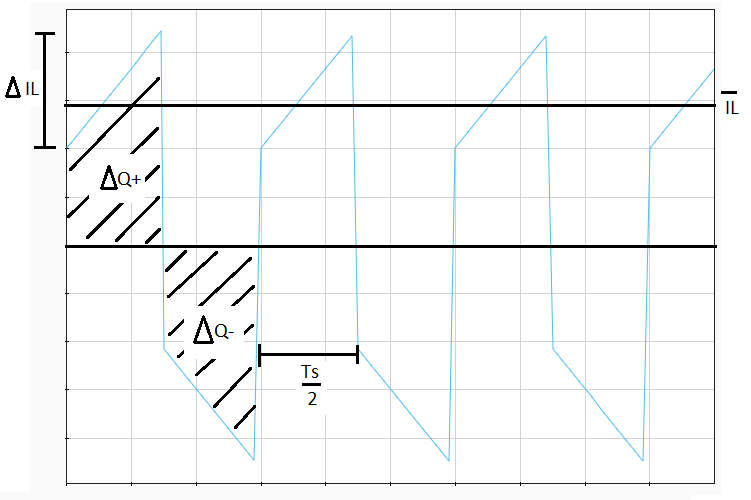
\includegraphics[scale=0.4]{Corriente-capacitores.png}
	\caption{Forma de onda de la corriente en C1 y C2.}
	\label{fig:img_ccorriente-capacitores}
\end{figure}

\noindent Por el electroimán circula una corriente media de 21 A en condiciones normales de trabajo. Por lo tanto, la carga del capacitor se puede calcular como:

\begin{equation} 
	\begin{aligned}
   	\Delta Q &= \int I dt\\	
	\Delta Q ^+ &= \frac{T_S}{2}*\Delta I_L * \frac{1}{2} + (<I_L> -\frac{\Delta I_L}{2})*\frac{T_S}{2}\\
	\Delta Q ^+ &= <I_L> *\frac{T_S}{2}\\
	\end{aligned}
\end{equation}

\noindent Con $\Delta I_L=500 \:mA$ y $T=0.47\:ms$ que corresponde a $Y = 2 \:mm$ según la tabla \ref{tab_mediciones}

\begin{equation} 
\Delta Q = 21\:A * \frac{0.47\:ms}{2} \approx 5\:mC
\end{equation}

\noindent Al considerar que un ripple de $\Delta V=500 \:mV$ es aceptable, se obtiene un valor de:

\begin{equation} 
	c = \frac{\Delta Q}{\Delta V} = 10 \:mF
\end{equation}

\noindent Para obtener este valor de capacidad utilizamos varios capacitores en paralelo para disminuir la ESR, como se muestra en la figura \ref{fig:img_capacitores-fuente}. Esto es porque por los capacitores circula una corriente de hasta 21.25 A. Por lo tanto, al colocarlos en paralelo se reduce la corriente que circula (en partes iguales), por cada capacitor:
\colorbox{yellow}{Tratar de redactar mejor}

\begin{figure}[H]
	\centering
	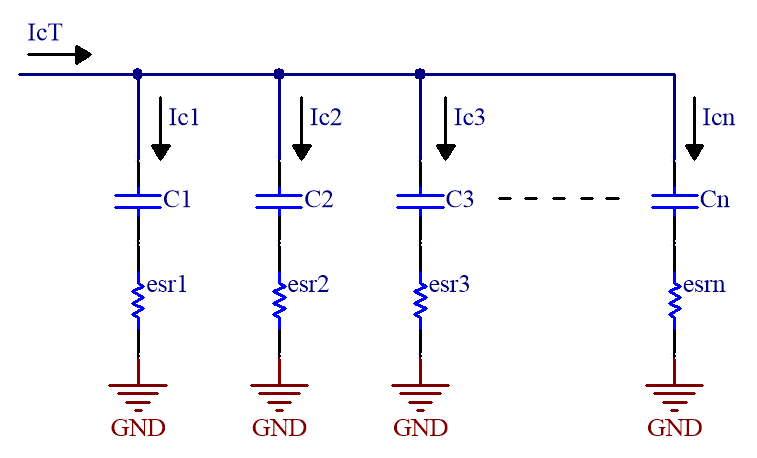
\includegraphics[scale=0.5]{Capacitores-fuente.png}
	\caption{Capacitores de la fuente.}
	\label{fig:img_capacitores-fuente}
\end{figure}


\begin{equation} 
	C = C1 + C2 + ... + C_n
\end{equation}


\noindent Si todos los valores de ESR son iguales obtenemos

\begin{equation} 
R_T = \frac{R_{ESR}}{n}
\end{equation}

\noindent Por lo tanto reemplazando se puede calcular la potencia que disipan como:

\begin{equation} 
	P = I^2 * R_T = 21.25^2 * \frac{R_{ESR}}{n}
\end{equation}

\noindent Se decidió utilizar 6 capacitores  de 2200 uF/50V con una ESR de 17 $\Omega$ (datos obtenidos de \cite{EKY-350ELL222MM25S}) . Por lo tanto reemplazando en la ecuación 4.4 se obtiene que la potencia disipada es de: 

\begin{equation} 
	P=1.28 W
\end{equation}


\subsubsection{Conmutación de alta frecuencia para el bootstrap}

\noindent Cuando el mosfet driver recibe una entrada que activa un MOS del lado superior, este comienza a cargar el gate con ayuda de la tensión que brinda el capacitor de bootstrap asociado a ese MOS. El capacitor de bootstrap entrega energía durante la carga del gate y durante todo el tiempo que el MOS esté activo (debido a la resistencia $R_{GS}$). Para poder recargar el capacitor, debe esperarse a que el driver reciba la entrada necesaria para apagar el MOS. Debido a que la implementación del driver de corriente utiliza un controlador por histéresis, no es posible asegurar que haya una conmutación en un periodo regular.

\noindent Para poder asegurar un periodo de conmutación constante y conocido se agrega un bloque que superpone una conmutación de alta frecuencia a la señal de control que ingresa al mosfet driver. De esta manera se producen conmutaciones en un intervalo regular y se cargan regularmente los capacitores de bootstrap. 

\noindent Se adopta una frecuencia de conmutación auxiliar de 50KHz y se hace variar el ciclo de trabajo de la salida del comparador con histéresis entre dos valores. Durante la carga del inductor, el ciclo de trabajo será del 90\% mientras que durante la descarga será del 10\%.

\noindent Para generar esta conmutación se agrega el oscilador que se observa en la figura \ref{fig:img_frecuencia-auxiliar} a la salida del comparador con histéresis. La frecuencia de conmutación se puede obtener en función de C1 como:

\begin{equation} 
	F_{aux} = \frac{4.5*10^{-5}}{C1} [Hz]
\end{equation}


\noindent Esta frecuencia debe ser mucho mayor a la fundamental de la corriente triangular para evitar problemas en el funcionamiento del sistema y, además, debe ser lo suficientemente alta para poder ser filtrada sin inconvenientes en la etapa de estimación de posición. Por lo tanto, al adoptar una frecuencia auxiliar de 50 KHz, resulta en C1= 900 pF.

\begin{figure}[H]
	\centering
	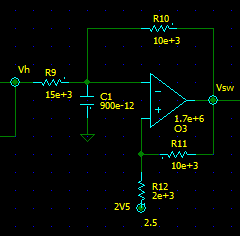
\includegraphics[scale=1]{Frecuencia-auxiliar.png}
	\caption{Circuito oscilador de frecuencia auxiliar.}
	\label{fig:img_frecuencia-auxiliar}
\end{figure}


\subsubsection{Simulación del sistema con oscilador auxiliar}

\noindent En la figura \ref{fig:img_corriente-auxiliar} se muestran las formas de onda obtenidas considerando el oscilador auxiliar necesario para el funcionamiento del bootstrap. 

\begin{figure}[H]
	\centering
	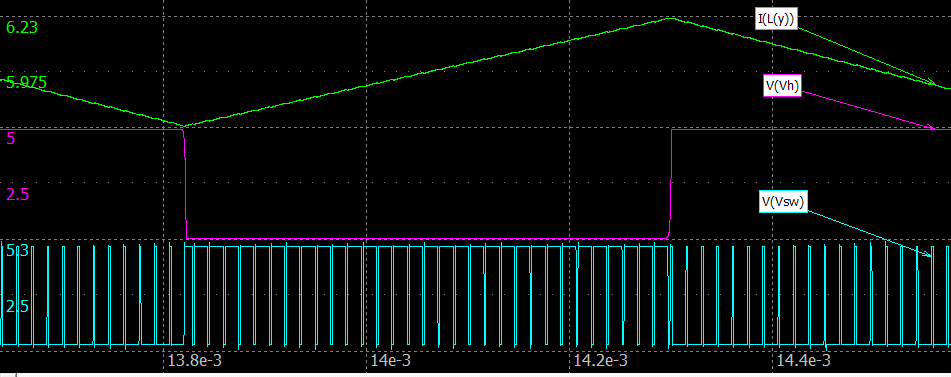
\includegraphics[scale=0.3]{Corriente-auxiliar.png}
	\caption{Simulación de corriente en el electroimán, salida del comparador, y conmutación auxiliar.}
	\label{fig:img_corriente-auxiliar}
\end{figure}

\subsection{Características estáticas y dinámicas del controlador}

\subsubsection{Corriente media del electroimán}

\noindent Para saber la corriente media que habrá a la salida con cierta tensión de entrada, se utiliza la transferencia de lazo cerrado (sin considerar polos, y suponiendo una alta ganancia de lazo abierto):

\begin{equation} 
	I_L = V_{i\_ref} * \frac{K_{in}}{H(s)} = V_{i\_ref} * 6 \frac{A}{V}
\end{equation}

\subsubsection{Frecuencia de conmutación de la corriente}

\noindent La frecuencia de conmutación del sistema se obtiene con:

\begin{equation}\label{eq_frec-sw} 
f_{SW} = \frac{V_{BUS}}{2*\Delta I_L * L(y)}
\end{equation}

\noindent Para $y = 4 mm $ se tiene una inductancia $L(4mm) = 16.44 mHy$ , lo cual resulta en una frecuencia $f_{SW }= 1460 Hz$ .

\subsubsection{Ancho de banda del controlador}

\noindent La dinámica del controlador, al depender de la inductancia, lo hace también del gap de aire. El ancho de banda (o velocidad con que responde) está limitado por la constante de tiempo del inductor con su resistencia serie. Juntas forman un sistema lineal de primer orden, con un polo en:

\begin{equation} 
	f_{polo} = \frac{1}{2\pi * L(y)}
\end{equation}

\noindent Al convertirlo a frecuencia angular:

\begin{equation} \label{eq_frec-angular}
	\omega _{polo} = \frac{1}{2\pi * L(y)}
\end{equation}

\noindent Tomando las condiciones del problema con Yo = 4mm, L = 7.55 mHy + 8.89 mHy, y Rl=0.2$\Omega$ el polo se ubica:

\begin{equation} 
	\omega _{polo} = \frac{0.2}{16.44 mHy} = 12.17 r/s
\end{equation}

\noindent La Tabla 4.2 muestra  entre qué valores de frecuencia se verá afectada la forma de onda al modificarse la distancia de separación.

\begin{equation} \label{eq_DeltaT}
	\Delta T [s] = \frac{\Delta I_L * (L(y) + L_{\infty})}{V_{BUS}}
\end{equation}


\noindent Considerando Rl=0.2 $\Omega$ 

\noindent En la ecuación \ref{eq_DeltaT}, $\Delta T$ representa el tiempo de crecimiento o de decrecimiento de la rampa de corriente (despreciando la resistencia del bobinado) en torno al valor nominal. El doble de este tiempo es igual al periodo de la corriente triangular $(2*T=\frac{1}{F_{SW}})$.

\noindent Según las mediciones de inductancia realizadas y aplicando las ecuaciones \ref{eq_frec-sw}, \ref{eq_frec-angular} y \ref{eq_DeltaT} se armó la tabla \ref{tab_mediciones}.


\begin{table}[H]
	\begin{center}
		\begin{tabular}{| c | c | c | c | c |}
			\hline
			Y[mm] & L(Y)[mHy] & $\Delta$ T[ms] & $f_{SW}$[Hz] & $\omega _{polo}$[r/s]\\ \hline
			0 & 76.45 & 1.59 & 313.93 & 2.62\\ \hline
			1 & 33.42 & 0.70 & 718.13 & 5.98\\ \hline
			2 & 22.64 &	0.47 & 1,060.07 & 8.83\\ \hline
			3 &	18.8 & 0.39 & 1,276.60 & 10.64\\ \hline
			4,4 & 15.5 & 0.32 & 1,548.39 & 12.90\\ \hline
			5,2 & 14.7 & 0.31 & 1,632.65 & 13.61\\ \hline
			6,5 & 14.4 & 0.30 & 1,666.67 & 13.89\\ \hline
			8,23 & 12.4 & 0.26 & 1,935.48 & 16.13\\ \hline
			inf & 8.89 & 0.19 & 2,699.66 & 22.5	\\ \hline
		\end{tabular}
		\caption{Valores calculados y medidos en función del Gap de aire.}
		\label{tab_mediciones}
	\end{center}
\end{table}

\subsection{Transferencia lineal del controlador de corriente}

\noindent En la ecuación \ref{eq_TLC-cc} se muestra la transferencia linealizada del controlador de corriente.

\begin{equation} \label{eq_TLC-cc}
TLC_{CC} = \frac{6}{1+\frac{s}{\omega _{polo}}}
\end{equation}

